% BEGIN TEMPLATE
\documentclass{article}
\usepackage{graphicx}
\usepackage{hyperref} 
\usepackage{xcolor}
\usepackage{nameref}
\usepackage{listings}
\usepackage{float}
\usepackage[title]{appendix}
\usepackage[ruled]{algorithm2e}
\graphicspath{ {../../images/} }
\bibliographystyle{acm}
% CHANGE THESE
\newcommand{\courseListing}{CSCI 8920}
\newcommand{\courseName}{Fundamentals of Deep Learning}
\newcommand{\assignmentTitle}{Homework Assignment \#1}
\newcommand{\assignmentSubtitle}{Dataset Processing Functions}
\usepackage{geometry}
\geometry{margin=1in}

\hypersetup{
    colorlinks,
    linkcolor={red!50!black},
    citecolor={blue!50!black},
    urlcolor={blue!80!black}
}
\urlstyle{same}
\definecolor{codegreen}{rgb}{0,0.6,0}
\definecolor{codegray}{rgb}{0.5,0.5,0.5}
\definecolor{codepurple}{rgb}{0.58,0,0.82}
\lstdefinestyle{mystyle}{
    commentstyle=\color{codegreen},
    keywordstyle=\color{magenta},
    numberstyle=\tiny\color{codegray},
    stringstyle=\color{codepurple},
    basicstyle=\ttfamily\footnotesize,
    breakatwhitespace=false,         
    breaklines=true,                 
    captionpos=b,                    
    keepspaces=true,                 
    numbers=left,                    
    numbersep=5pt,                  
    showspaces=false,                
    showstringspaces=false,
    showtabs=false,                  
    tabsize=2
}

\lstset{style=mystyle}

\begin{document}
  \begin{center}
  
\includegraphics[scale=0.15]{UNO-Logo-Color.png}
  \\[0.3in]
  \textbf{\courseListing{}}\\
  \courseName{}
  \\[0.75in]
  \textbf{\assignmentTitle{}}\\
  \assignmentSubtitle{}
  \\[0.75in]
  \textbf{Patrick Davlin}
  \\[0.75in]
  \textbf{Computer Science Department}\\
  \textbf{Peter Kiewit Institute}\\
  \textbf{University of Nebraska}
  \\[0.75in]
  \textbf{Spring 2021}
  \\[0.3in]
  
\includegraphics[scale=0.075]{UNO-Icon-Color.png}
  \newpage
\end{center}
  \graphicspath{{./images/}}
% END TEMPLATE
\section{Introduction}
A critical component of any deep learning project is developing an intimate understanding of the data upon which that project will act.
One thing learned last semester in the Advanced Applications class is that there is no model of any sophistication that can be run on random data; every project is unique and requires careful selection and assembly for training data.
Speaking generally, models are developed around two different sets of data-- \textit{training} and \textit{testing} (or \textit{validation}) data.
In this assignment, several different methods of organizing training and validation data were implemented for comparison:
\begin{itemize}
    \item \textbf{Holdout}: splitting a dataset directly into training/validation sets (generally, 70/30, respectively);
    \item \textbf{K-Fold Cross-Validation}: dividing a dataset into several groups, then rotating through each single group as the validation data, while remaining groups are training data;
    \item \textbf{Bootstrapping}: generating datasets of a set length randomly, with replacement; and,
    \item \textbf{Batch generation}: generating datasets of a set length sequentially, using data from the start of the dataset to "fill in" if the end of the dataset is reached.
\end{itemize}


\section{Project Setup} \label{setup}
At the end of the CSCI 8110 course, I was able to obtain a new Nvidia GTX 3080 card.
At the time, the CUDA 8 architecture on the card was not well-supported, so assignments needed to be done on a combination of personal hardware (Windows) and online applications (Paperspace Gradient or Google Colab).
Months later, Tensorflow has substantially better support for newer cards.
On a full re-install of Windows, Tensorflow was up and running in under an hour without any trouble.
As such, this assignment was done entirely on a local machine using the following specific packages:
\begin{itemize}
    \item Python 3.8.6 
    \item Tensorflow 2.4.1
    \item Matplotlib 3.3.4
\end{itemize}.

\section{Implementation} \label{impl}
\textit{Note: this section discusses sections of code; the entire project can be found in the \nameref{codelist}}.
\subsection{Loading CIFAR10 Data}
The first task for the assignment was to load and output CIFAR10 data:
\begin{lstlisting}[language=Python]
# Load CIFAR10 data
(cifar10_data, _), (_, _) = cifar10.load_data()
cifar10_data = cifar10_data / 255

# Display sample images
plot_cifar_img(cifar10_data)
\end{lstlisting}
To confirm, the resulting images are below:

\begin{figure}[H]
    \centering
    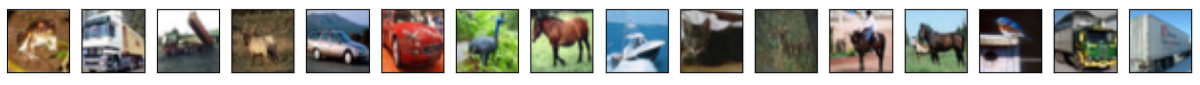
\includegraphics[width=6in]{csci-8920/hw-1/images/8920-hw-1-cropped.png}
    \caption{CIFAR-10 images}
    \label{fig:data}
\end{figure}

\subsection{Holdout}
Implementing the first three methods (Holdout, K-Fold, and Bootstrapping) was a fairly straightforward exercise.
Being listed first, and being the most straightforward, the holdout function was implemented as a simple way to create a pre-defined split of the provided data:
\begin{lstlisting}[language=Python]
def holdout(data_in,training_pct=0.7):
  num_records_in_training_set=int(len(data_in) * training_pct)
  np.random.shuffle(data_in)
  training_data = data_in[0:num_records_in_training_set]
  validation_data = data_in[num_records_in_training_set:]
  return training_data, validation_data
\end{lstlisting}

For a dataset with 50,000 entries, like the CIFAR-10 data, the split comes out to 35,000 training images and 15,000 testing images.
Output confirming this is available in the \nameref{completeout} Appendix.

\subsection{K-Fold Cross-Validation} \label{kf}
Implementing K-folds required some thought about how to properly divide records into groups.
Dividing evenly is easy; 50,000 images in five groups yields even groups of 10,000 images, but dividing the same 50,000 images into six groups would leave two images unused.
With this in mind, it was important to add the "remainder" records to groups, taking care to keep them as even as possible:
\begin{lstlisting}[language=Python]
def k_folds(data_in, num_groups, validation_set_index):
  np.random.shuffle(data_in)
  leftover_records_as_divided = len(data_in) % num_groups
  num_records_in_k_group = math.floor(len(data_in)/num_groups)
  k_groups = []
  previous_k_slice = 0
  for i in range(num_groups):
    k_slice = previous_k_slice + num_records_in_k_group
    if i < leftover_records_as_divided:
      k_slice = k_slice + 1
    k_group = data_in[previous_k_slice:k_slice]
    k_groups.append(k_group)
    previous_k_slice = k_slice
\end{lstlisting}

To extend the example, dividing 50,000 images into six groups would provide four groups of 16,666 images and two groups of 16,667 images, creating an even sum of 50,000 total images.

After dividing the inital dataset into groups, the next task is to designate one as the validation set and combine the remaining groups into a training set, then return both:
\begin{lstlisting}[language=Python]
  training_set = np.array([])
  for i in range(len(k_groups)):
    if i == validation_set_index -1:
      validation_set = k_groups[i]
    else:
      if training_set.size == 0:
        training_set = k_groups[i]
      else:
        training_set = np.concatenate((training_set,k_groups[i]))
  return training_set, validation_set
\end{lstlisting}
Again, complete output confirming this is available in the \nameref{completeout} Appendix.

\subsection{Bootstrapping}
The bootstrapping process felt, generally, more vague than other methods.
Not much clarity was developed around what parts of the input set would qualify as validation sets once needed, so a general sampling method was developed:
\begin{lstlisting}[language=Python]
def bootstrap(data_in, batch_size, num_batches):
  bootstrap_datasets=[None] * num_batches
  for i in range(num_batches):
      bootstrap_datasets[i] = []
      np.random.shuffle(data_in)
      random_indices = generate_random_numbers(batch_size, len(data_in))
      for j in random_indices:
          bootstrap_datasets[i].append(data_in[j])
  return bootstrap_datasets
\end{lstlisting}

Of note, the \lstinline{generate_random_numbers()} method generates an array of random numbers without worrying whether any number appears twice, to adhere to the "with replacement" requirement in bootstrapping.
This general method allows for any size data to be returned, up to the input dataset's length, and any number of randomly-sampled batches.

\subsection{Batch Generator}
The difficult part of this implementation was mostly in understanding how python generators work; the use of the \lstinline{yield} statement was not immediately intuitive given my relative lack of experience with Python.
After some looking around online the intuitive way of thinking of it was to consider the generator function as a constant loop where the \lstinline{yield} statements represent specific points in time where data should be exported from the function.
With this in mind,the general approach seemed to be to iterate through a batch worth of records and yield that batch until the end of the data input was reached.
When that limit is reached, the program checks to see whether there is any data queued to be returned and, if so, add data from the beginning of the array to the leftover data and yield it.
Then, the data for the next iteration is started to offset the amount of data added. 
This can repeated any number of times, as shown below:
\begin{lstlisting}[language=Python]
def batch_generator(data_in, batch_size):
  offset = 0
  overflow_data = [] 
  while True:
      offset = 0
      if len(overflow_data) > 0:
          offset = batch_size - len(overflow_data)
          print('data wraparound occurred here; pulling {} records from front'.format(offset))
          yield np.concatenate((overflow_data, data_in[0:offset]))
          overflow_data = []

      for x in range(offset, len(data_in), batch_size):
          output_data = data_in[x : x + batch_size]
          if len(output_data) != batch_size:
            overflow_data = output_data
          else:
            yield output_data
\end{lstlisting}

\subsection{K-fold Generator}
With an understanding of generators in hand, the next obvious extension was to implement a generator for the K-fold algorithm.
The general thought process behind this is that the K-fold generator is based on the idea of folding through data by setting each group, sequentially, as the "validation set".
The code for the generator, then, performs the same logic as described in the \nameref{kf} subsection, adjusted instead to iterate through each group to set it as the validation data.
For brevity, and since it is largely repeated from the prior K-fold implementation, this code is omitted here, but can be read in its entirety in the \nameref{codelist} section.

\section{Results \& Observations} \label{observations}
Being fairly straightforward (at least in terms of deep learning projects) there is relatively little to say here.
These implementations are, admittedly, fairly rudimentary.
The K-Fold implementation is rather slow when dealing with a larger number groups, which is compounded in generator form.
The bootstrap implementation, since it's generating a random array of integers and then filling new arrays with data from those indices, is similarly slow.
Optimizing these operations would go a long way toward improving the runtime of many Keras models implemented on to train and validate the data they return.
Without a thorough understanding of Python packages and tooling, though, it isn't clear where those time savings can be achieved.

\section{Conclusions}
Having extensively used Keras models in CSCI 8110, without thinking of the ways that datasets are used in training and validating those models, made this assignment much more valuable.
Oftentimes in that class, models I implemented were "thrown" together without much of an eye toward the quality or organization of data being used as a basis upon which the model would operate.
As a basis for improving my ability to develop and maintain good data, this exercise represents facets of machine learning training that are valuable to consider, even when letting frameworks do the work of organizing data for me.

\newpage
\begin{appendices}
\section{Complete Program Output} \label{completeout}
\lstinputlisting{hw-1-out.txt}
\section{Complete Code Listing} \label{codelist}
\lstinputlisting[language=Python]{hw-1.py}
\end{appendices}
\end{document}